\section{Technical Overview}
A simplified overview of the overall setup is provided in \autoref{fig:overview} as a block diagram. The setup is physically located at the department of Control and Automation at Aalborg University in the laboratory. The figure is structured with the highest abstraction layer at the top (i.e. the ROS (Robotic Operation System)) environment which establish a wireless TCP/IP communication channel receiving all positions from the robot as feedback. It produces likewise positioning control signals to the NI (National Instruments) single board RIOs (Reconfigurable Input/Output) which handles all input/output communication from the user. The NI single board RIOs consist of a primary and a secondary board. The reason for having two RIO boards is solely the lack of input/outputs on one board.

The RIO boards direct the control signals to a cascaded controller taking in a velocity reference and delivers a current control signal to the ESCON motor driver. The velocity and current controller are implemented in hardware (FPGA) to ensure sufficient controller speed relative to the system [artikkel]. 

The lowest layer is located in the bottom, i.e. the actuators in form of seven Maxon motors. 
\begin{figure}[H]
	\center
	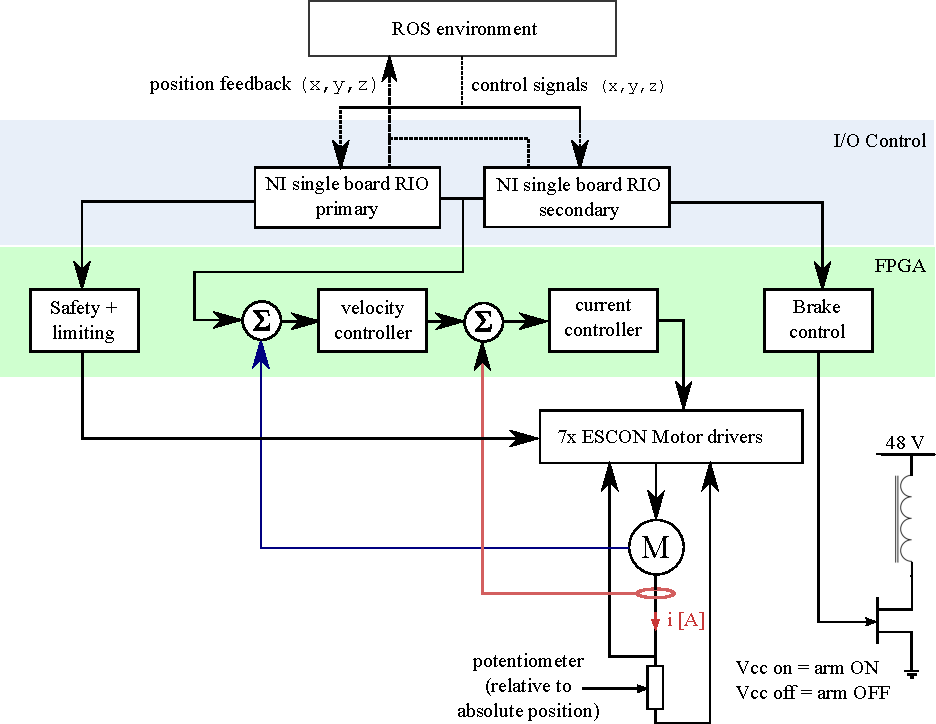
\includegraphics[width=0.95\textwidth]{overview.pdf}	\caption{This is a nice figure. Here illustrated for hand roll master.}
	\label{fig:overview}
\end{figure}
The focus of this thesis is the highest abstraction layer, i.e.the ROS environment.
